Existem dois limites até onde é possível acertar o laser: os pontos extremos do espelho $E_1$ e $E_2$. Todos os pontos dentro da região entre esses dois extremos podem ser alcançados pelo laser, como pode ser visto no exemplo abaixo, com a região destacada em azul:

\begin{center}
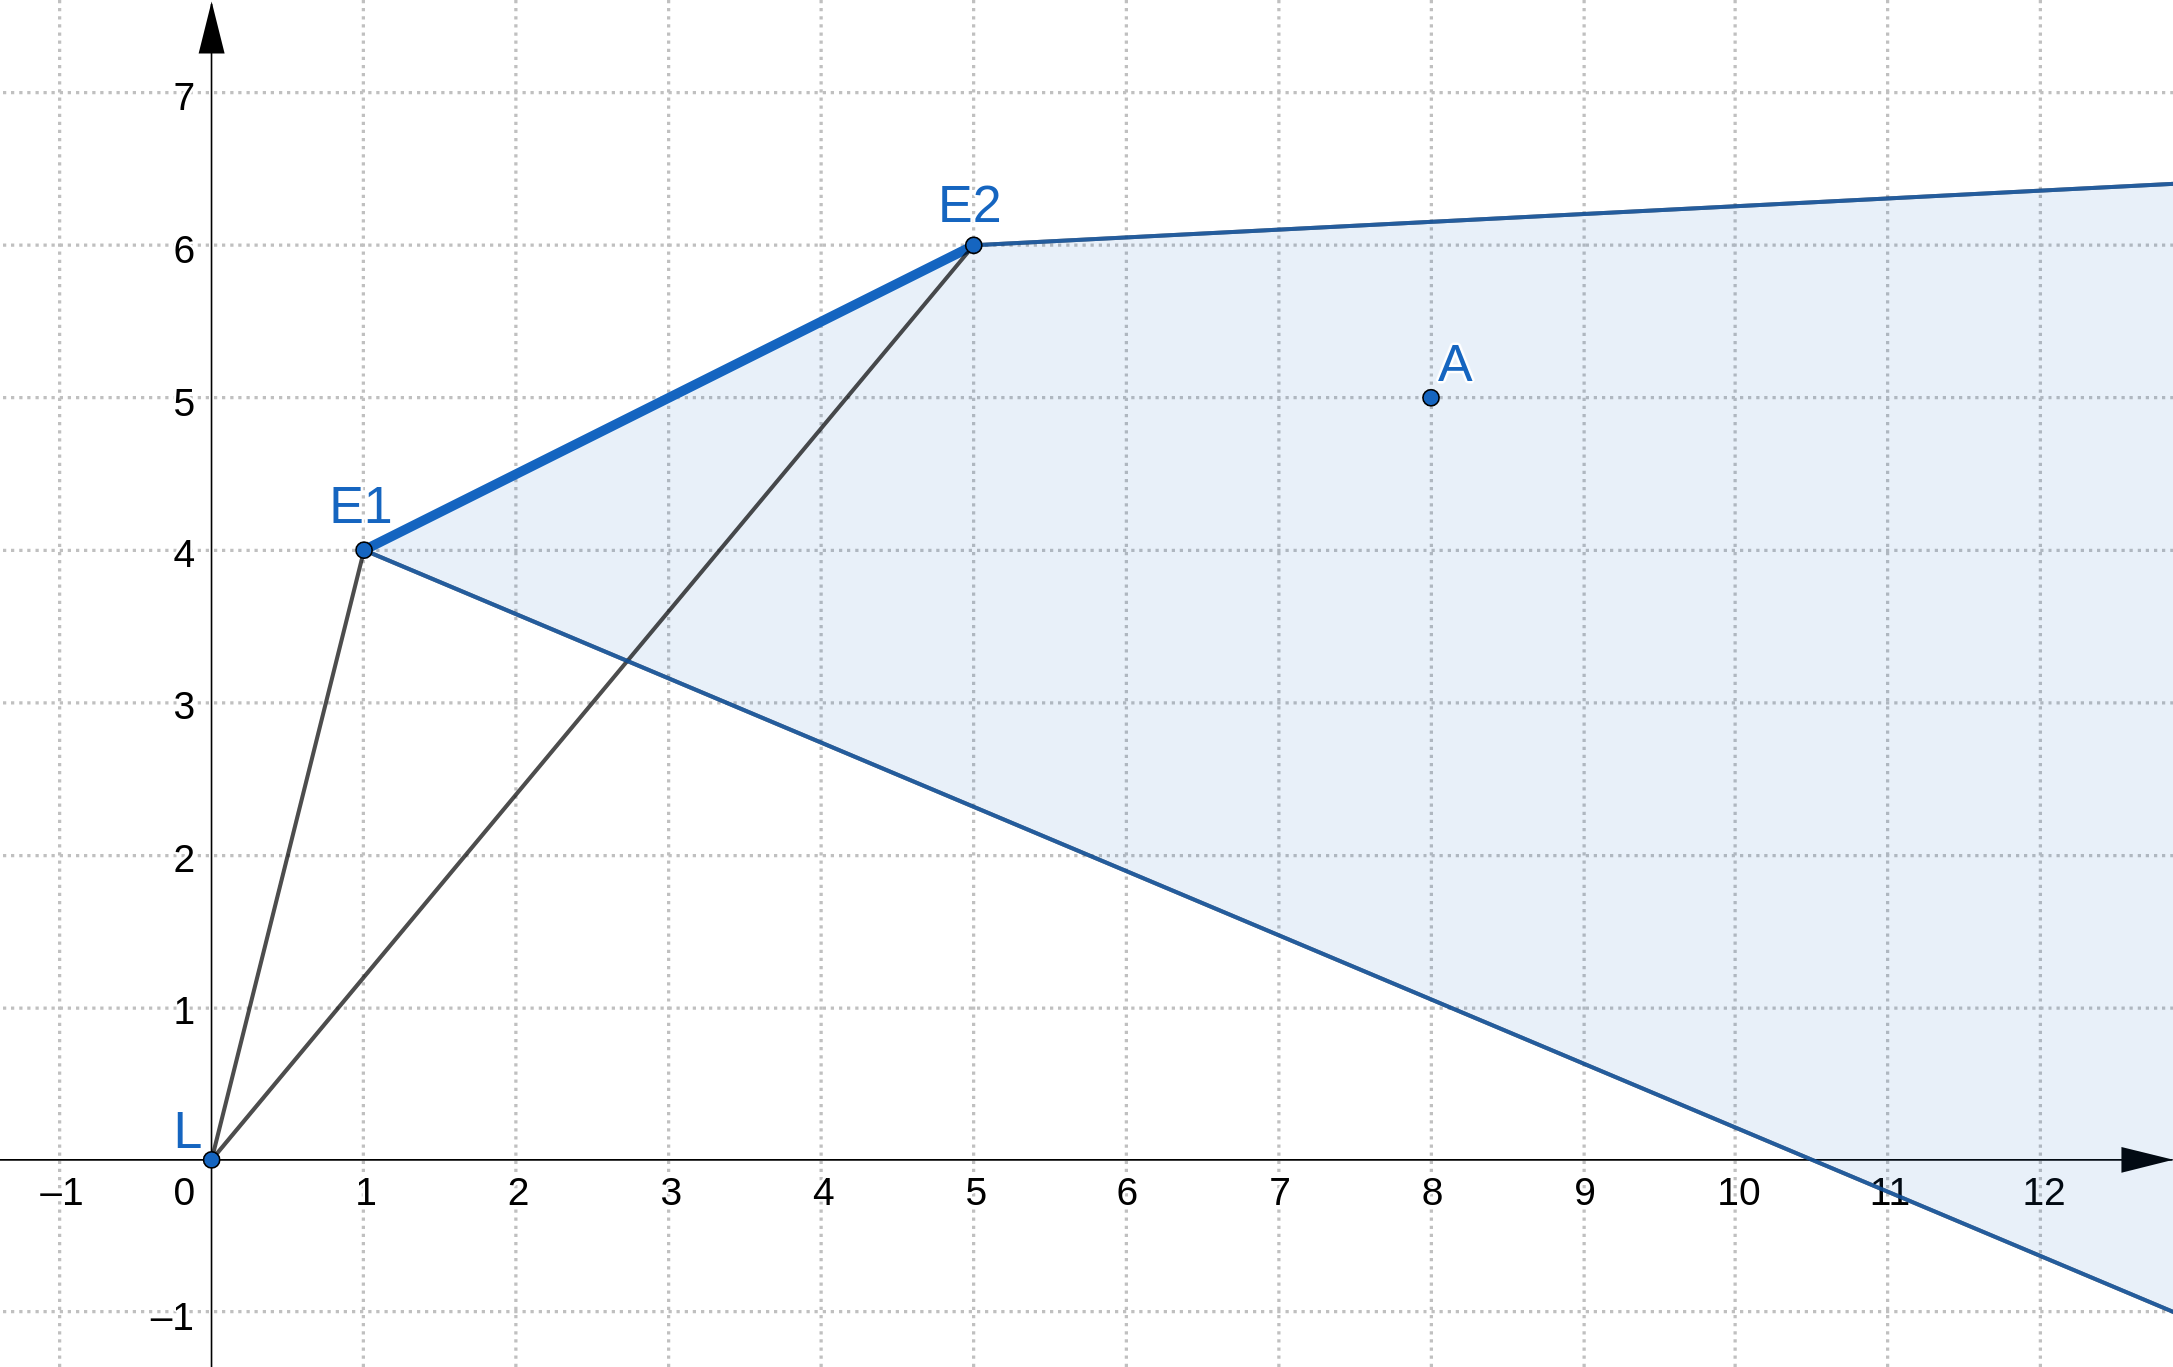
\includegraphics[width=13cm, height=9cm]{tutorial1.png}
\end{center}

Logo, a solução consiste em saber se o ponto $A$ está dentro dessa região. O espelho respeita as leis da física, que regem a reflexão da trajetória do laser ao bater no espelho ($\theta_i = \theta_r$). Existem algumas formas de simular essa reflexão, é possível rotacionar a reta que representa a trajetória do laser, é possível rotacionar o espelho para que fique paralelo a um dos eixos coordenados, contudo são abordagens que exigem uma implementação mais complexa.

A solução descrita a seguir utiliza somente das operações vetoriais \textbf{Produto Vetorial} e \textbf{Produto Escalar}, juntamente com a ideia de \textbf{Imagem Virtual}: ao invés de refletir o laser, vamos gerar a imagem virtual $A_m$ do ponto $A$ para dentro do espelho, sendo agora possível considerar que o laser não reflete no espelho, apenas entra para dentro de sua imagem virtual, almejando agora acertar o ponto $A_m$.

\begin{center}
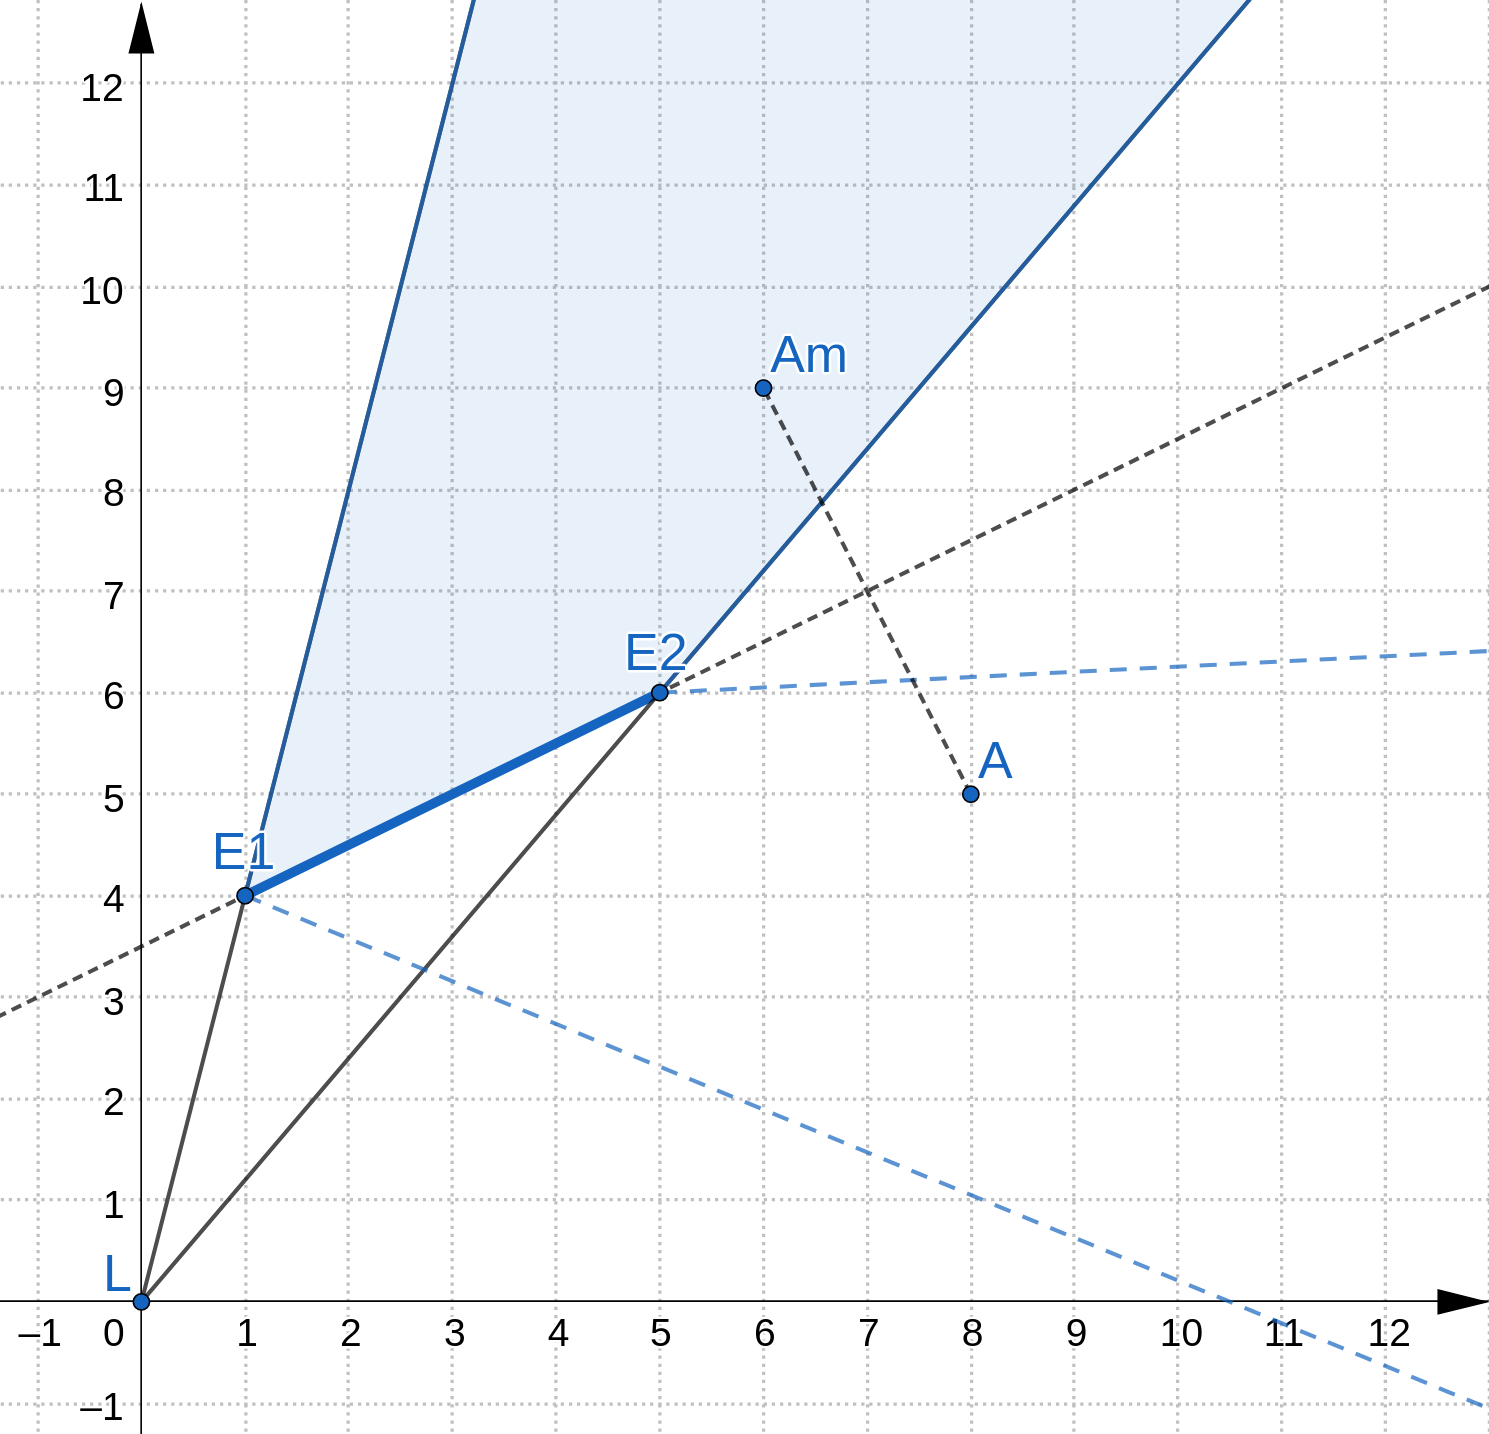
\includegraphics[width=11cm, height=11cm]{tutorial2n.png}
\end{center}

Para gerar a imagem virtual $A_m$, basta espelhar/refletir o ponto $A$ em relação a reta do espelho de forma simétrica, utilizando da operação produto escalar. A partir do produto escalar é possível encontrar a projeção do ponto $A$ na reta do espelho, com isso, utilizamos de soma e subtração de vetores para refletir o ponto para o outro lado da reta, centrado na projeção encontrada.


Uma vez com o ponto $A_m$ calculado, basta identificar se esse ponto está entre as retas $LE_1$ e $LE_2$, e para isso é possível utilizar da operação produto vetorial. A partir do sinal do produto vetorial é possível identificar se um ponto está para a direita, para a esquerda ou colinear com uma dada reta. Caso o ponto esteja para a esquerda/direita das duas retas (sinal dos produtos vetoriais sejam iguais), ele não está entre as duas retas e não pode ser alcançado, caso contrário (sinal dos produtos vetoriais sejam diferentes), o ponto se encontra entre as duas retas e é possível atingi-lo como o laser.


Caso queira aprender mais sobre o produto vetorial e escalar, assista as aulas da Turma Avançada disponíveis no link \url{https://unb-cic.github.io/Maratona-Extensao/avancado/geometria/}